\chapter{Tutorial}

This tutorial will introduce you to the most common features of Tremolo-X by guiding you through a variety of example simulations.
It is assumed that you read the chapter ``First Steps'' prior to starting with this tutorial.

All files mentioned here already exit in your Tremolo-X home directory in the folder \texttt{tutorial}. The leading number in the folder name corresponds to the section number in this chapter.

\section{Optimizing an initial particle setup}
Very often the setup of a simulation requires the assembly of a data file (with the particle positions) by hand or script.
As a result the particle distribution is almost always non-optimal in the sense that the relative positions create local energy spikes
which adversely affect the stability and equilibrium property of the simulation.

To counter these effects a simulation is usually preceded by an optimization phase, in which particle positions are slightly modified towards a (static) energy minimum.

We demonstrate the optimization procedure for an argon gas with reduced units.

We start by writing up the file \texttt{argon.tremolo}

\begin{lstlisting}
global: defaultpath=".";
global: projectname="argon";
global: comment="Reduced argon example";
global: systemofunits=custom;
\end{lstlisting}

First we set the \texttt{defaultpath}. Even though we do not intend to use an external path to files in this example, this must always be set.
In the second line we provide the \texttt{projectname}, all files for this simulation \textit{must} carry this name (input) or respectively \textit{will} carry this name (output).
The \texttt{comment} can be freely used to add information about the simulation.
In the last line we specify that we will use a custom system of units. This means that we have to specify a few base magnitudes, from which any others are
derived. Those magnitudes are specified by line pairs, the first fixing the physical unit to be used, whereas the second specifies the amount:

\begin{lstlisting}
custom: lengthunit=angstrom;
custom: lengthscalingfactor=3.4;
custom: timeunit=ps;
custom: timescalingfactor=2.17;
custom: massunit=u;
custom: massscalingfactor=39.948;
custom: currentunit="e/s";
custom: currentscalingfactor=1;
custom: temperatureunit=K;
custom: temperaturescalingfactor=120;
\end{lstlisting}
In the above example,
a length unit corresponds to $3.4 \angstrom$, whereas mass is measured in $39.948$ atomic mass units. (Thus a length of $2$ in Tremolo-X units is $6.8\angstrom$, whereas a
Tremolo-X mass of $0.5$ corresponds to $19.974u$.
\bigbreak
Now we turn to the particles and their potentials, those are specified in the \texttt{argon.potentials} file.
First we specify the particle types present in the simulation. In this case we use only one particle, which we name Argon, with chemical symbol \texttt{Ar}. The element name
appears in some of the output files. Then we fix the \texttt{sigma, epsilon, sigma14 and epsilon14} values~\cite{ArgonLJ1987}. (Generally you should keep to the convention \texttt{sigma = sigma14} and \texttt{epsilon = epsilon14}, unless you have parameter sets for complex molecules which tell you otherwise.) Those are used in the computation of various potentials, namely the
Lennard Jones potential which we will use here.
\begin{lstlisting}
particles       {
        particle:       particle_type=Argon,    element_name=Ar,        sigma=1,        epsilon=1,      sigma14=1,      epsilon14=1,    mass=1, free=3, charge=0;
        };
\end{lstlisting}
Due to our custom choice of units, all those values are set to one.
The same holds true for the particle mass. Degrees of freedom are three (this is the norm), the particles hold no charge.
In the same file we enter the actual potentials to be used in between particles. Since only one type of particle is present there are not many mixtures to keep track of.

\begin{lstlisting}
nonbonded_2body_potentials      {
        lennardjones:   particle_type1=Argon,   particle_type2=Argon,   r_cut=12.0;
        ljspline:       particle_type1=Argon,   particle_type2=Argon,   r_cut=12.0,     r_l=10.0;
        };
\end{lstlisting}

We denote the pair of particle types which are affected by the potential. For the first Lennard Jones potential we specify a cut of radius $r_{cut}$ of $12.0$\todo{Why?} (custom units),
outside of which the interaction between two particles is set to 0. Since that introduces a discontinuity, we also second potential, which is a splined Lennard Jones Potential.
It gets an additional parameter $r_l$, after which a spline is used to interpolate from the current value to 0 a $r_{cut}$.
Note that both types of potentials are full LJ potentials in their own right. Using both would cause approximately twice the normal potential (and twice the normal forces) to be calculated
between particles. Nevertheless, it does not hurt to supply any applicable potentials in this file, as they can be switched on and off at a different location,
determining those which contribute to the particle interaction.

This location is the \texttt{argon.validates} file.
\begin{lstlisting}
validate: particle_type=Argon, state=on;

validate: force_type=lennardjones, state=off;
validate: force_type=ljspline, state=on;
\end{lstlisting}
Here we validate the use of the particle type ``Argon'' and decide which of the two potentials shall remain in effect, while making sure that the other one is switched off.

The majority of parameter choices are made in the \texttt{argon.parameters} file. Here we will determine the domain, the number of optimization steps
and make choices about the output created by the program.
First we state that this simulation is to be an optimization, not a dynamic simulation.:
\begin{lstlisting}
integration: type=optimization;
\end{lstlisting}

Next we determine the domain as cubic shaped with a side length of 81.05. The borders are to be periodic,
so a particle leaving the cube over one side will reenter it via the other.
\begin{lstlisting}
domain {
    size: type=cube, size=81.05;
    border: bt_xlow=periodic, bt_xhigh=periodic, bt_ylow=periodic, bt_yhigh=periodic,
        bt_zlow=periodic, bt_zhigh=periodic;
};
lcs: cellrcut=12.0;
\end{lstlisting}
The choice of the cell size (\texttt{cellrcut}) is more algorithmic that geometric, but we have to ensure that \texttt{cellrcut < size}.\\
Remark: In the parallel case this condition changes to
\texttt{
\begin{equation*}
\text{cellrcut} < \frac{\text{size}}{\# \text{ of processors per dimension}}.
\end{equation*}}

In the next block we set the options for parameterization. In this example we want to optimize particle positions only.
Optimization is to be done by conjugate gradient (cg) method with 2001 steps (for algorithmic reasons the step number must be divisible by 3, otherwise it would be adjusted upwards).
\begin{lstlisting}
optimization {
    particle: state=on, alpha=0.2, beta=0.8, lambda1=0, lambda2=1;
    common: algorithm=cg, maxcg=2001, RT=periodical, maxresetcg=6, LS=strongwolfe, maxlinesearch=6, mean_force_eps=1e-6, mean_force_eps_rel=1e-10, prefactor=1e-4;
};
\end{lstlisting}

The CG method is reset periodically to speed up convergence and furthermore we use strong Wolfe conditions on the cg line search.
\texttt{mean\_force\_eps} and \texttt{mean\_force\_eps\_rel} are the cutoff values for the absolute and relative mean force values respectively.
The last parameter in line \texttt{prefactor}, is possibly the most important, as it directly controls the size of changes.
Depending on the energy surface of the sample, a small value might be imperative to prevent the optimization from failing.
On the other hand a small value prevents significant changes and slows the method down.
\bigbreak
In the last block of this file we specify the type and intervals of output created. \notiz{What is meant by visuals?} Visuals shall be created every 5 time units or 10 iteration steps, whereas the particle data shall be written every 500 time units or 10 iteration steps. Any other measured quantities are written every 0.5 time units or after 1 iteration step.
In this example we measure only energy.
\begin{lstlisting}
output {
    Outvis: T_Start=0, T_Delta=5.0, Step_Delta=10;
    Outdata: T_Start=0, T_Delta=500, Step_Delta=10;

    Outm: T_Start=0, T_Delta=0.5, Step_Delta=1;

    energy: measure=on;
};
\end{lstlisting}

\bigbreak
The last item missing before we can start the simulation is the \texttt{argon.data} file supplying the initial particle positions. This file may not contain any free comments, all lines must match a particular format. Here we display only the first few lines of the file:
\begin{lstlisting}[escapechar=']
# ATOMDATA Id x=3 u=3 type
# INPUTCONV temp 2.7
1       80.10823        14.25174        47.74411        0.0     0.0     0.0     Argon
2       70.29545        7.599451        58.29292        0.0     0.0     0.0     Argon
3       66.10589        2.939586        69.22116        0.0     0.0     0.0     Argon
4       77.18604        63.33052        73.03413        0.0     0.0     0.0     Argon
5       76.02857        54.41654        24.62265        0.0     0.0     0.0     Argon
6       16.96877        11.43903        21.40026        0.0     0.0     0.0     Argon
7       53.09684        7.723396        47.48021        0.0     0.0     0.0     Argon
8       77.50526        70.68508        49.97302        0.0     0.0     0.0     Argon
 '$\vdots$'
\end{lstlisting}
The first line sets the layout of the particle list. It always begins with
\texttt{\# ATOMDATA} followed by the attributes set in the file. In this case
this is the particle id, the particles position (3 columns), the particles
velocity (3 columns) and the particle type. As you can see we already supply
spatial coordinates, however we set all velocities to zero. Those will be set
by the other \texttt{\#} preceded line in the file, which performs some
manipulation on the data provided. Such lines always begin with \texttt{\# INPUTCONV}.
In this instance we set the temperature of the sample. Using a Maxwell-Boltzmann distribution
each particle is then assigned a random velocity.\footnote{Note that if you plot these
distributions, you see the shape of a Maxwell-Boltzmann distribution, but you seldomly
find the parameters to be matching exactly. This is due to finite size effects, even
very large simulations contain few particles compared to the real world, where you
might have particle numbers by the mol.} The
temperature is measured in the unit system we provided in the \texttt{argon.tremolo} file.

Now all pieces are in place to start the optimization on our particles.
You can use the commands you learned in the ``Quickstartguide'' (chapter \ref{Quickstart}) to run the optimization.

The optimized particle positions are written to \texttt{argon.data.999}. \fehler{a '9' is missing in the file name}
The file looks very much like the original data file, though we find that
the \texttt{INPUTCONV} line has been removed and two lines have been added
at the top (Their use is explained in section~\ref{sec:domain_opt}). Furthermore the velocity columns now show non-zero entries -
particle speeds corresponding to the specified temperature.

\subsection{Exercises}
\begin{itemize}
\item Increase the prefactor to $1.0e^{-2}$. What happens? The message tells you which particle causes the problem - have a look at it and the surrounding particles in the data file.
\item Have a look at the potential energy curve, how does it behave?
\end{itemize}

\section{Setting up a basic simulation}
Now we are ready to start the actual simulation. Fortunately we did most
of the work required setting up the optimization, so we now only have to
amend very few lines in the \texttt{argon.parameters} file and make sure
that we use the optimized data instead of the original.
First we need to change the line specifying the integration type from ``optimization'' to ``dynamics'':
\begin{lstlisting}
integration: type=dynamics;
\end{lstlisting}
 The \texttt{cellrcut} and \texttt{domain} blocks remain untouched.
 We could remove the block with the optimization parameters, but since
 we changed the integration type to dynamic (removing optimization), we can also leave it in place without harm.

However we need to add a new block, setting the parameters for the dynamics:
\begin{lstlisting}
dynamics {
    ensemble: ensemble=NVE;
    propagator, verlet: delta_T=0.5e-3, endtime=1000;
};
\end{lstlisting}
Here we set particle \textbf{n}umber, domain \textbf{v}olume and total
\textbf{e}nergy to be constant (NVE ensemble). For the integration of the
particle trajectories we choose a standard \texttt{verlet} algorithm with a
time step of $0.005$ custom time units. The total simulation time will be 1000 custom time units. \fehler{Do you mean $0.0005$ or is this a mistake in the listing above?}

At last we make a small addition to the \textbf{output} block; we would like to gain some insight into the velocity distribution of the particles:

\begin{lstlisting}[escapechar=']
 '$\vdots$'
energy: measure=on;

    analyze {
        velocity: measure=on, meanmeasure=off, vis=off, min=0.0, max=25.0, n_bin=50;
    };
};
\end{lstlisting}
After the \texttt{energy} line we add a sub-block for analysis (within the output block).
We consider velocities between 0 and 25 (custom units) and use bins of 0.5 (custom units) each.

Now we have to make sure that we use the optimized data instead of the original.
(As a general rule one should keep copies of the original at all times.) So,
after having copied the original \texttt{argon.data} file somewhere safe,
we rename the \texttt{argon.data.9999} file as \texttt{argon.data}.
For this example we can still ignore the extra lines. \notiz{Which extra lines?}

Now you can start the simulation as we did with the optimization before.

\subsection{Exercises}
\begin{itemize}
\item Compare the values of the \texttt{argon.etot, argon.ekin} and \texttt{argon.epot} files (plot them in the same graph). What do you notice?
\item Take a look at the velocity distribution in the \texttt{argon.histogram} file. \notiz{Is there something particular one have to look at?}
\item Try starting the simulation with the original data instead of the optimized.
\item In order to smooth measurement curves and remove static, one often uses mean measurements over intervals. Switch mean measurements on for the energy measurements and compare the curves of the mean measurement with those of the regular measurement (they are written to separate files.)
\item Have a look at the different energy curves. Then, in the \texttt{argon.data} file, change the temperature value to 3.0. (Use the \texttt{\#INPUTCONV temp} line from the previous lesson.) The individual velocity values are then overwritten. How does this affect the different energies?
\end{itemize}


\section{Using the Berendsen thermostat}
In this section we will introduce the first of two different thermostats. Given the previous preparations we require even less changes to the parameter file. All changes are within the \texttt{dynamics} block.

First we have to change the ensemble type:
\begin{lstlisting}
dynamics {
    ensemble: ensemble=NVT;
    propagator, verlet: delta_T=0.5e-3, endtime=1000;
\end{lstlisting}
Instead of the total energy, we now hold the \textbf{t}emperature constant. For this type of thermostat the propagator remains untouched.
Then we open a new sub-block for the details of the thermostat:
\begin{lstlisting}
    thermostat {
        berendsen: state=on, T_Interval=0.01;
        constanttargettemp: state=on, T_Temp=2.5;
    };
};
\end{lstlisting}
We declare that we use the \texttt{berendsen} thermostat and choose to enforce it every second time step by our choice of \textbf{T\_Interval}.
Furthermore we declare that we wish to hold the temperature constant and at which value. Note that we chose a value lower than
the originally set temperature (regardless of whether you did the exercise or not.)
Those are all the changes required, so go ahead and run the simulation. \notiz{which data file has to be used? The one with '9999' after running the last simulation?}

In difference to the previous example, where the temperature varied around its original value, you will observe a very sharp drop
from the original to the designated temperature. Afterwards all temperature values hit the value almost \textit{exactly}. In
fact, every second one is exactly at 2.5, whereas every other varies ever so slightly. 

\subsection{Exercises}
\begin{itemize}
\item Compare the values of the \texttt{argon.etot, argon.ekin} and \texttt{argon.epot} files (plot them in the same graph). What changed compared to the previous lesson?
\item Play with the time interval for the thermostat. Make it match the propagator timestep or make it a thousand times as long and observe the effects. In addition to the kinetic energy, observe the potential and total energy as well.
\end{itemize}

\section{An alternative: The Nose-Hoover-thermostat} \notiz{Shouldn't it be a é?}
We also introduce a second type of thermostat. Three lines require a change in order to switch to the alternative, all in the \texttt{dynamics} block of the \texttt{argon.parameter} file.
\begin{lstlisting}
dynamics {
    ensemble: ensemble=NVT;
    propagator, beeman2v: delta_T=0.5e-3, endtime=1000;
\end{lstlisting}
Here we have to make a change to the propagator, in order for the Nose-Hoover thermostat to work, a velocity integrator is required. \notiz{What is a velocity integrator?}
\begin{lstlisting}
    thermostat {
        berendsen: state=off, T_Interval=0.01;
        nosehoover: state=on, F_Mass=1.0;
        constanttargettemp: state=on, T_Temp=2.5;
    };
};
\end{lstlisting}
Instead of deleting the \texttt{berendsen} line we can also switch it off. \notiz{In the tutorials-file F\_Mass is set to 5.0...}
In the added \texttt{nosehoover} line we do not have to specify an interval
for the thermostat, but a virtual mass. This constant determines the strength
of the coupling of the particles in the simulation with a virtual heat bath. \notiz{I am not sure what this is supposed to mean...}

Start the simulation as before and observe the temperature behavior.

You will note that the temperature oscillates, first significantly reducing
its amplitude. While the amplitude increases again after some time it does
not gain the same value as before. Thus, when using the Nose-Hoover thermostat
considerations with respect to equilibration are imperative. \notiz{I do not understand the last sentence.}

\subsection{Exercises}
\begin{itemize}
\item Again, compare the values of the \texttt{argon.etot, argon.ekin} and \texttt{argon.epot} files (plot them in the same graph). What changed compared to the previous two lessons?
\item Play around with different virtual masses (0.01 - 100.0) and different starting temperatures. You will note some different behaviors.
\end{itemize}


\section{Optimizing the domain}
\label{sec:domain_opt}
Sometimes it is not possible to determine the optimal size of the domain
prior to the simulation. In addition to the use of the barostat which we
handle in the next lesson of this tutorial, we will now take a look at the
initial optimization

We begin by modifying the the optimization of the sample prior to the actual \fehler{Duplicate 'the'.}
simulation. In particular we allow that, in addition to the positions of
the atoms, also the box may be scaled to minimize the potential energy.

In the \texttt{argon.parameters} file from the first lesson we add two lines
to the optimization block
\begin{lstlisting}
optimization {
    particle: state=on, alpha=0.2, beta=0.8, lambda1=0, lambda2=1;
    simucell: state=on, alpha=0.2, beta=0.8, lambda1=0, lambda2=1;
    simucell: constraint=isotropic, XX=1, YY=1, ZZ=1, XY=0, XZ=0, YX=0, YZ=0, ZX=0, ZY=0;
\end{lstlisting}
where we set the line search parameters for the cell optimization (generally we can use the same parameters as for the particle positions) and
may also choose some constraints on which entries of the box matrix are allowed to vary.

Finally, we make one addition to the \texttt{common} parameter set by adding an external pressure value:
\begin{lstlisting}
    common: algorithm=cg, maxcg=2001, RT=periodical, maxresetcg=6, LS=strongwolfe, maxlinesearch=6, mean_force_eps=1e-6, mean_force_eps_rel=1e-10, prefactor=1e-4, extpressure=0.0024455185;
};
\end{lstlisting}

After running the optimization, take a look at the file \texttt{argon.data.9999}. In addition to the new coordinates of the particles you find a time stamp and a box matrix entry. This is the domain shape after the optimization has finished. To make use of these values, you need to transfer them to the parameter file, as described in the next lesson.

\subsection{Exercises}
\begin{itemize}
 \item Change the \texttt{extpressure} value. Check and compare the new box values\footnote{If you run tremolo with increased verbosity (e.g. \texttt{-v} the new box matrix - among other things - will be written to the standard output)}. (Changes by order of magnitude are advised for clearly visible results.)
 \item In the constraint matrix, change one of the main axis entries (\texttt{XX, YY, ZZ}) to 0. Check and compare the new box values.
 \item Change one of the secondary axis entries to 1.
  Check and compare the new box values. Now rename the constraint to \texttt{constraint=standard} and check again.
  Repeat the process for \texttt{constraint=symmetric}.
\end{itemize}


\section{Introducing barostats}
\label{tutorial:barostat}
In some cases it is desired to run simulations not only with isothermic, but also isobaric conditions.
For this to be possible we allow the volume of the box to be variable and set a barostat similarly to the thermostat.

Again we work in the \texttt{argon.parameter} file and enter the thermostat after (or in place of) the thermostat:
\begin{lstlisting}
dynamics {
    ensemble: ensemble=NPE;
    propagator, beeman2v: delta_T=0.5e-3, endtime=1000;

    thermostat {
        berendsen: state=off, T_Interval=0.01;
        nosehoover: state=off, F_Mass=0.01;
        constanttargettemp: state=off, T_Temp=2.5;
    };

    barostat {
        parinello: state=on, f_mass=1;
        constantpressure: state=on, Pressure=0.0024455185;

        constraint: type=isotropic;
        constraintmap: xx=1, yy=1, zz=1, xy=0, xz=0, yx=0, yz=0, zx=0, zy=0;
    };
};
\end{lstlisting}
In the first line we switch the barostat on and specify a virtual mass.
In the second line we can choose whether the pressure aimed at shall be constant and if so, at what value. Note that as usually this value is in reduced units.
Furthermore, we make our choice of constraints on the allowed changes to the box. First we specify a specific type of constraint, and afterwards we can apply
additional modification by specifying entries in the box-matrix which may be affected.

Finally we have to deal with the particle data. If we start with a file where we did not use the box-optimization there is nothing else to worry about, we can start
the simulation immediately. But lets take the \texttt{argon.data.9999} file from the previous lesson. (Preferably the one which was optimized with the originally supplied parameters.) Should you attempt to start it right away, you will receive an error
message. This is due to the fact that the box-matrix in the data file and the one in the parameter file are different. So go ahead and change the domain in the
appropriate line. (Note that the value shown here may be different from your value. If you wish to use a different result (e.g. the one won from \texttt{symmetric}
constraints) you need to change the domain type as well. For the appropriate syntax see~\ref{sub:domain}.

\begin{lstlisting}
domain {
    size: type=cube, size=7.935811e+01;
    border: bt_xlow=periodic, bt_xhigh=periodic, bt_ylow=periodic, bt_yhigh=periodic,
        bt_zlow=periodic, bt_zhigh=periodic;
\end{lstlisting}


\subsection{Exercises}
\begin{itemize}
 \item Change the \texttt{extpressure} value. Check and compare the new box values. (changes by order of magnitude are advised for clearly visible results)
 \item In the \texttt{constraintmap}, change one of the main axis entries (\texttt{XX, YY, ZZ}) to 0. Check and compare the new box values.
 \item In the \texttt{constraintmap}, change one of the secondary axis entries. Check and compare the new box values.
 \draft{\item Change the \texttt{f\_mass} value to 1000. Check and compare the of the box values.}
 \item Go back to the previous lesson and use one of the other constraints types (such as standard). Now transfer this \texttt{argon.data.9999} file and insert
 its domain shape in the \texttt{argon.parameter} file. For the appropriate syntax see~\ref{sub:domain}.
\end{itemize}

\section{Bonded potentials and measuring bonds}
Hitherto only the nonbonded Lennard Jones interaction has been covered in
this Tutorial. In most cases the connectivity of atoms is known and it
is desired that it stays in its initial configuration. In these cases
the indices of the neighbor atoms are set in the appropriate column in
the data file and bonded potentials are specified in the
\texttt{.potentials} file. The bond type covered here, named
\texttt{bond} is a harmonic potential -- computationally inexpensive and
with unbreakable bonds. As
per definition bonded-type bonds can't be broken, however with harmonic
potentials there will be a restoring force proportional to the
deflection from the minimal energy distance $r_0$. While unphysical for
large displacements, this behaviour can also be desired if simulations
are carried out under very high kinetic energies to speed processes up,
because the general structure of the molecules will persist.

\begin{center}
    
\includegraphics[width=5cm, height=3cm]{visuals/butane} % 300 dpi
\end{center}

We will set up a butane example and measure the bond distances in the
CH3- and CH2-groups. There are three atom types: Methyl-carbon
(\texttt{C} in CH3), methylene-carbon (\texttt{Ci} in CH2, i stands for
``inner'') and Hydrogen (\texttt{H}). The butane data file is build
accordingly and the field \texttt{neighbors=4} is added. The ensemble
provided with the tutorial files consists of $5\times 5\times 5$ butane
molecules with a density of \SI{2.71}{\kilogram\per\cubic\meter}. The
unit system used is kcalpermole.

\begin{lstlisting}[caption=Header of the .data file]
# ATOMDATA Id type x=3 u=3 neighbors=4
\end{lstlisting}

When setting up the \texttt{butane.potentials} file, begin with Lennard
Jones interaction, which should additionally work in between molecules.
Tremolo-X handles Lennard Jones in bonded molecules in a way, that the
potential is \emph{not} calculated among direct neighbors. However for
large molecules, like proteins, intramolecular interaction should be
considered: These are controlled via the settings \texttt{sigma14} and
\texttt{epsilon14}, as they take effect from the fourth bond on, hence
the naming.

As for the bonded potentials we use \texttt{bonds}, \texttt{angles} and
\texttt{torsions}. The angle potential, like the bonds, is harmonic
(linear restoring force for angle displacement from an optimal value)
and the torsional potential is expressed as cosine series expansion. All
parameters are taken from the AMBER94 force field. For the literal
definition of the potential terms see the potentials-section in this
manual (\ref{sse:bondedpotentials}).

\begin{lstlisting}[escapechar=', caption=Excerpt from the
    .potentials file]
bonds {
  bond: particle_type1=C, particle_type2=Ci, bond_type=harmonic, k_b=310, r_0=1.526;
  '[\dots]'
};

angles {
  angle: particle_type1=C, particle_type2=Ci, particle_type3=Ci, angle_type=harmonic, k_th=40, theta_0=109.5;
  '[\dots]'

torsions {
  torsion: particle_type1=H, particle_type2=C, particle_type3=Ci, particle_type4=H, torsion_type=cosine, k_1=1.4, delta_1=0, n_1=3, mult=1;
  '[\dots]'

};
\end{lstlisting}

The simulation \texttt{\$PROJECTNAME.parameters} are a simple \texttt{NVE} ensemble
with verlet propagator and initial temperature of \SI{0}{\celsius}. In the
\texttt{analyze} section bond distance measurement is set up. It
doesn't matter whether the measured pair is bonded in means of the
\texttt{neighbors} field: Every pair with specified types undershooting the
specified threshold (in this particular case \SI{180}{\pico\meter} for C--C and
\SI{140}{\pico\meter} for H--C) are considered bonded and their Ids written to the
\texttt{\$PROJECTNAME.info.bonds} (vis) file. The mean value of bond lengths of any 
pair of types requested in the \texttt{\$PROJECTNAME.parameters} file is written to 
the \texttt{\$PROJECTNAME.generalmeas} file.

\begin{lstlisting}[caption=Excerpt from the .parameters file]
    analyze {
        bond: measure=on, meanmeasure=off, vis=off;
        bondDistances {
            bondDistance: particle_type1=Ci, particle_type2=Ci, distance=1.8;
            bondDistance: particle_type1=C, particle_type2=Ci, distance=1.8;
            bondDistance: particle_type1=Ci, particle_type2=H, distance=1.4;
            bondDistance: particle_type1=C, particle_type2=H, distance=1.4;
        };
\end{lstlisting}

As we can see the mean values oscillate around a constant, so there is
no time dependant development. We assume the ensemble is equilibrated
after 20 time units and compare the mean of the mean values for any
available pair and get following results:

\begin{center}
    \begin{tabular}{ccc}
        \toprule
        Bond & Distance/\si{\pico\meter} & $r_0$/\si{\angstrom} \\
        \midrule
        \texttt{C}--\texttt{Ci} & 152.7(1) & 1.526 \\
        \texttt{Ci}--\texttt{Ci} & 152.7(2) & 1.526 \\
        \texttt{C}--\texttt{H} & 109.1(1) & 1.09 \\
        \texttt{Ci}--\texttt{H} & 109.08(9) & 1.09 \\
        \bottomrule
    \end{tabular}
\end{center}

There are no differences in the bond length within statistical error and
the values match the $r_0$-Parameter because the same parameters were
used for both, inner and outer, carbon atom types. The nearest neighbors
of the atoms (spatial configuration) are not taken into account thus
leading to an identical bond distance.

\subsection{Exercises}
\begin{itemize}
    \item Increase the temperature or lower the bond strength and
        observe the magnitude of the oscillation.
    \item Alter the equilibrium distance $r_0$.
\end{itemize}

\section{Tersoff potential and stress}
After we successfully introduced basic bonded and non-bonded force fields, this
chapter shows how to use a bond order potential to determine Young's Modulus of
a single graphene sheet. Instead of defining fixed individual neighbors, the
potential function will determine the spatial configuration of surrounding
carbon atoms by itself. This way the \texttt{graphene.data} file looks rather trivial,
the force field parameters for \texttt{graphene.potentials} are taken directly
from \cite{tersoff88a}:

\begin{lstlisting}
tersoff {
    tersoffparticle: particle_type=C0, A=32115.7, B=7990.67, lambda=3.4879, mu=2.2119, beta=1.5724e-07, n=0.72751, c=38049, d=4.3484, h=-0.57058, R=1.95, S=2.1;
};
\end{lstlisting}

Just like in \ref{tutorial:barostat} an \texttt{NPT}-ensemble is used, but this time
additionally to the external pressure we also support a custom stress tensor,
which stretches the domain in \texttt{xx}-direction with linearly increasing
strength, starting from $0$ in the beginning up to $1e5\,\frac{[F]\,[V]}{[A]}$\footnote{\textbf{F}orce, \textbf{V}olume and \textbf{A}rea.
For a detailed explanation of the volume term see chapter~\ref{output:stress}}
(\texttt{kcalpermole} units). At this time note that the stress value is not
given in units of pressure, as one would expect, but contains a surplus
$V$-Term.  The volume can usually be derived from the domain dimensions, but
particularly in this tutorial we have to \emph{decide} how much volume a single
graphene sheet has. Also the box vectors need to be changed individually, so we
will choose \texttt{standard} constraints (\texttt{isotropic} constraints would be
infeasible due to the coupling of the constraints).

\begin{lstlisting}
barostat {
    parinello: state=on, f_mass=500;
    constraint: type=standard;
    constraintmap: xx=1, xy=0, xz=0, yx=0, yy=1, yz=0, zx=0, zy=0, zz=0;
    constantpressure: state=on, Pressure=1.45742e-05;

    stresstensor: [time, stress, interpolation, xx, xy, xz, yy, yz, zz =
        (0, 0, linear, 1, 0, 0, 0, 0, 0),
        (200, 1e5, linear, 1, 0, 0, 0, 0, 0)];
};
\end{lstlisting}

Stress and strain are measured automatically if \texttt{outm} is set. However
if you are interested in the stress distribution along individual particles you
need to use the \texttt{local\_stress}-feature:

\begin{lstlisting}
analyze {
    local_stress: localstress=on;
};
\end{lstlisting}

If activated, the beta column in the visual .pdb output contains per particle
stress, which can be visualized with an external tool like VMD-Viewer (not
covered by this tutorial). Due to limitations of the PDB-format the numerical
value is clipped at $99.99\,\frac{[F]\,[V]}{[A]}$.

After the simulation has been finished, the output is analyzed by plotting a
stress-strain diagram. The strain is defined as the length change relative to
the initial box \texttt{xx}-length $L_0$: $\epsilon(L) = \frac{L-L_0}{L0}$.
The argument will be the $43^{rd}$ column in the file \texttt{graphene.mbox}, which
is the domain length in \texttt{xx} direction. The stress is read
from column 31 in the same file and divided by the volume of the graphene sheet, which is the product of
\texttt{xx} length (column 43), \texttt{yy} length (column 44) and
\textit{height}, which has to be chosen by the user. We set $height=3.7
\mathring{A}$, the inter layer distance in graphite. Note that since we pull,
the stress value from the file is negative. With this information we can now
use gnuplot to create the diagram and fit a slope against the initial
section, representing the elastic zone where Hook's Law applies. This slope is
the Young's Modulus.

\begin{lstlisting}
gnuplot> L0 = 48.19683
gnuplot> epsilon(L) = (L-L0)/L0
gnuplot> plot 'graphene.mbox' using (epsilon($43)):(-$31/($43*$44*3.7))

gnuplot> f(x) = E*x
gnuplot> fit [0:0.04] f(x) 'graphene.mbox' using (epsilon($43)):(-$31/($43*$44*3.7)) via E
\end{lstlisting}

\begin{figure}[h]
    \centering
    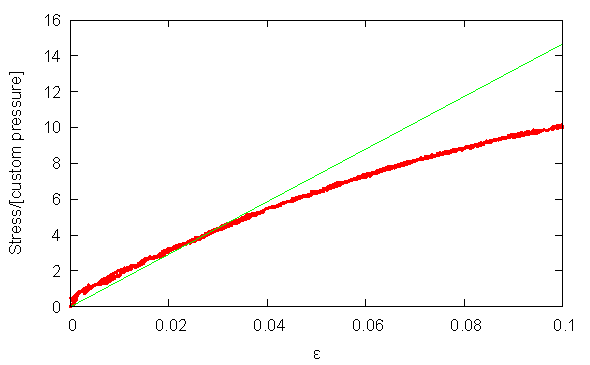
\includegraphics{visuals/graphene.pdf}
    \caption{Stress-strain diagram of monolayer graphene (red) with green slope fit.}
\end{figure}

We obtain $E=146.7(5)\,\frac{[F]}{[A]}$, in SI-units $1019(3)\,\textrm{GPa}$, which
sufficiently reproduces the measurement of $1\,\textrm{TPa}$ in~\cite{egraphene}.

\subsection{Exercises}
\begin{itemize}
    \item Change the pull direction to \texttt{yy}. Are there differences?
    \item Alter the force progression:
    \begin{itemize}
        \item Increase the simulation length by factor ten.
        \item Add a $100\,[t]$ relaxation time at the beginning ($\sigma=0$).
        \item Increase the maximum stress at the end of the simulation by factor five.
    \end{itemize}
    Create a new stain-stress plot -- is there a difference in the fit quality
    ($\chi^2_\textrm{d.o.f.}$ and parameter error as supplied by gnuplot)?
\end{itemize}

\section{Long ranged potentials 1 - Halley's Comet with $\mathbf{N^2}$}
This tutorial covers how to set up simulation to use long ranged
potentials like gravity or the coulomb potential. In either case the
potential's distance characteristic is $\propto\ 1/x$ and any kind of
cutoff introduces significant errors on the forces and with them error
in macroscopical observables.

The simpelest way to deal with these kind of potentials is using an
ordinary pair potential. As stated earlier the potential should not be
cut off but has to to fit the linked cell structure of the domain. With
only a few particles it is adequate to run the whole simulation in a
single cell, the performance drops quadratically with the particle
number. In this example we simulate our solar system and calculate when
Halley's Comet runs through its perihelion point next time (as of time
of writing, year 2013).

To obtain handy numbers we set up following unit system in the
\texttt{.tremolo} file:

\begin{center}
    \begin{tabular}{ccc}
        \toprule
        Quantity & Unit & Equals \\
        \midrule
        Length & \SI{1.496e11}{\meter} & \si{\astronomicalunit} \\
        Time & \SI{86400}{\second} & \siday \\
        Mass & \SI{1e23}{\kilogram} & $\approx m_\mathrm{Earth} / 100$ \\
        \bottomrule
    \end{tabular}
\end{center}

For the \texttt{.data} file we use positions (relative to the
Barycenter) and velocities obtained from JPL HORIZONS for sixty
astronomical objects of our solar system including the most massive
ones. The data represents the state of the solar system on December
19th, 2012.

Tremolo-X doesn't support ``gravity'' literally, but since the potential
is identic to the coulomb potential disregarding the force constant we
set up a coulomb simulation with adapted \texttt{epsilon0inv}. It can
easily be calculated with Gnu Units:
\begin{lstlisting}
> units -t G "(m*1.496e11)**3 / (kg*1e23 * (s*86400)**2)"
1.4881216e-11
\end{lstlisting}
Note that the value needs to be multiplied by $-1$ so equally named
``charges'' attract each other.

We use an NVE ensemble with \texttt{verlet} propagator,
\SI{0.05}{\siday} \texttt{timestep} and \SI{100}{\siyear} \texttt{endtime},
``temperature'' and ``pressure'' can't be applied on the experimental
conditions. Also it would not be accurate to wrap around the
gravitational forces at the borders of the solar system as it is
preferred when homogenous systems are observed, so we choose the domain
to three times larger than the solar system, place it in the center
(done with a \texttt{INPUTCONV SHIFT} directive in the data file) and
set \texttt{leaving} boundary conditions (particles passing the border
are removed):

\begin{lstlisting}
lcs: cellrcut = 80.0;

domain {
    size: type=cube, size=240;
        border: bt_xlow=leaving, bt_xhigh=leaving, bt_ylow=leaving,
    bt_yhigh=leaving, bt_zlow=leaving, bt_zhigh=leaving;
};
\end{lstlisting}

A single linked cell will be large enough to contain the whole
ensemble. This is not practical for large scale molecular dynamics
because it can't be paralellized, however unless a more sophisticated
method like SPME (covered in the next section) is used, it is the only
way to obtain accurate results using long ranged potentials.

The \texttt{coulomb} section is set up thusly:

\begin{lstlisting}
coulomb {
    permittivity: epsilon0inv=-1.4881216e-11;
    n2spline: state=on, r_cut=80, r_l=70, i_degree=5;
};
\end{lstlisting}

The \texttt{n2spline} solver calculates the force for every pair and cuts
off beyond \SI{70}{\astronomicalunit} with a spline taper (like
\texttt{ljspline}). The cutoff is chosen large enough to contain the
whole solar system so the forces will be exact. If \texttt{n2spline} is
used in molecular dynamics with small cutoff the spline interpolation
guarantees conservation of energy but the forces will be off their exact
result due to the characterstic of the potential.

The bond distance measurement covered earlier is used to measure the
distance between Halley's Comet/Earth and the Barycenter:
\begin{lstlisting}[escapechar=']
output {
'[\dots]'
    analyze {
        bond: measure=on, meanmeasure=off, vis=off;
        bondDistances {
            bondDistance: particle_type1=Barycenter, particle_type2=Earth, distance=80;
            bondDistance: particle_type1=Barycenter, particle_type2=Halley, distance=80;
        };
    };
};
\end{lstlisting}

Finally we set up the objects in the \texttt{.potentials} file. To
calculate the gravity potential with the coulomb solver we need to set
the ``charge'' of the particle to its mass. The Barycenter is included
as pseudo particle with mass 1 and no charge -- this way it won't be
affected by any force and stay central.

After running the simulation we extract the time to the minimum of
$|\vec r_\mathrm{Barycenter}-\vec r_\mathrm{Halley}|$ by plotting the
first and fourth column of the \texttt{.generalmeas} file. It's 17750
time units (days), so the next perihelion is 25th July 2061, slightly
deviant to the value computed with HORIZONS: 28th July. This relative
difference of 0.02\% is caused by the simplification of the solar system
to sixty objects and the resulting difference in the local density. The
minima of the Earth--Barycenter distance are \SI{365.24}{\siday} apart
which matches the definition of the tropical year.

\subsection{Excercises}
\begin{itemize}
    \item Remove any particle but Sun, Jupiter, Barycenter and Halley
        and compare the relative error of the perihelion.
    \item Only remove Jupiter from the original setup and compare the
        relative error, observe planetary trajectories and the length of an
        earth year.
\end{itemize}


\section{Long ranged potentials 2 - Sodium chloride with SPME}
This part covers a typical usage scenario of coulomb forces in molecular
dynamics with more than just a few particles. To maintain a good
performance with a large $N$ the potential is seperated into a short
ranged part, which is calculated in a linked cell fashion as before, and
a long ranged part, which is calculated by Ewald summation in fourier
space, to take into account farther particles. In comparison to the Fast
Multipole Method, which abstracts groups of far particles into a single
one, this way is espacially suitable for periodic systems, like an ionic
crystal: In this example we are going to simulate solid NaCl and measure
its radial distribution functions. The system
of units used is \texttt{kcalpermole}.

In the \texttt{.potentials}-file we set up the short ranged interactions
using the Tosi Fumi\cite{tosifuminacl} Potential, which has shown to
produce accurate results with this kind of system. The starting
configuration in the data file is an NaCl-structure with small random
offset for each atom at \SI{20}{\celsius}.

We set up an \texttt{NPT}-ensemble in the \texttt{.parameters} file with
\SI{1000}{\hecto\pascal} pressure maintained by the Parrinello-Barostat with
isotropic constraint (the crystal is cubic) and
Nose-Hoover-Thermostat for fixed temperature. In the
\texttt{coulomb}-section we specify the parameters for the
\texttt{spme}-method and a force constant using the vacuum permittiviy:

\begin{lstlisting}
coulomb {
    permittivity: epsilon0inv=332;
    spme: state=on, r_cut=9.0, G=0.32, i_degree=5, cellratio=4;
};
\end{lstlisting}

Up to \texttt{r\_cut}, which is the short ranged part of the potential,
the force is evaluated locally (restricted to neighbored cells) and pair
wise, as if \texttt{n2spline} was used. From there it is approximated by
bell curves with splitting coefficient
\texttt{G}, which is inverse to the standard deviation $\sigma$, and
applied on a mesh, which is created by splitting the linked cell
\texttt{cellratio} times (rounded upward to the next power of two).
\texttt{G} should be kept at \SIrange{0.24}{0.35}{\angstrom^{-1}}.

In the \texttt{analyze}-section we set up the measurement of the radial
distributions of all atom types:

\begin{lstlisting}[escapechar=']
output {
'[\dots]'
    analyze {
        radial: measure=on, meanmeasure=off, vis=off, r_cut=9.0, n_bin=50;
        radialdistribution {
            radialdist: particle_type1=Na, particle_type2=Na;
            radialdist: particle_type1=Na, particle_type2=Cl;
            radialdist: particle_type1=Cl, particle_type2=Cl;
        };
    };
};
\end{lstlisting}

The value of \texttt{r\_cut} has to be within the \texttt{lcs: cellrcut}
limits, just like the \texttt{r\_cut} of the potentials.

Since we now use the SPME method, we have to use a parellel version
of Tremolo-X, since the SPME method is not implemented sequentially.
Nevertheless you can unse the SPME method and start the parallel 
version with a single process.

\emph{If you do not know how to run the parallel version of Tremolo-X,
please check chapter \ref{FirstParallelSteps} and \ref{running_tremolo}.}

\subsection{Excercises}
\begin{itemize}
    \item Compare the radial distribution histograms from first (ideal
        NaCl structure) and last timestep.
    \item Decrease/Increase the temperature and observe the differences
        in the radial distribution.
\end{itemize}

\section{Melting point of Sodium Chloride}
In the previous Tutorial the basics for simulating an ionic crystal
using the Coulomb- and Tosi-Fumi-Potential have been covered while this
one shows how to determine the melting point of NaCl, which is a common
application of molecular dynamics. From the different methods described
in \cite{nacl_melting} we are going to use the \emph{Voids method}: A
series of NaCl lattices with increasing defect concentration (removed
atoms) is simulated using an NPT-ensemble with temperature timeline.
Starting with an ideal lattice, which is a hypothetical, defect free
state at \SI{0}{\kelvin}, the temperature at which the lattice breaks
(``melting point'') is significantly overestimated because the
activation energy for this transition is very high. By removing atoms
from the crystal it becomes labile and the lattice breaks easily if the
temperature is high enough, lowering the activation energy to start the
melting process. If the defect concentration is too high the crystal
rearranges back into a more stable configuration, increasing the
observed melting point. This process leads to a reduced volume which has
to be compensated for, using a barostat. Therefore if the measured melting point is
plotted against defect concentration one can see that the measured melting point
decreases quickly with increasing defect concentration at first and then
oscillates around the actual melting point, which can be obtained by
calculating the mean value.

A tricky aspect is how to observe the melting point: Liquid and solid
state can be discriminated using the MSD-measurement, potential energy,
density, radial distribution or bond length, usually indicated by a rapid
slope change which can be seen if these measurements are plotted.
Preliminary studies have shown that observing the bond lenght is the
easiest to interpret while very accurate option in this particular
example: As the crystal heats up the bond lenght increases linearily
until the crystal breaks and the bond distances relaxes rapidly. The
obsverved melting point $T_m$ is the temperature at maximum bond lenght.

The simulation setup is similar to the previous tutorial apart from the
thermostat settings and more measurement options in the
\texttt{nacl.parameters} file:

\begin{lstlisting}[extendedchars=\true, inputencoding=utf8x]
thermostat {
    timeline: state=on, [time, temperature, interpolation =
    (0, 0.5822, linear), # 20C°
    (100, 0.5822, linear),
    (1000, 2.9255, linear)]; # 1200C°

    nosehoover: state=on, F_Mass=800;
};
\end{lstlisting}
\todo{Buchstabendreher beim Gradzeichen im PDF/Text fixen
(Encodingproblem mit lstlisting).}

With these settings the temperature is held constant at
\SI{20}{\celsius} for 100 time units and then lineary increased to
\SI{1200}{\celsius} at the end of the simulation (1000 time units).

\begin{lstlisting}
bond: measure=on;
bondDistances {
    bondDistance: particle_type1=Na, particle_type2=Cl, distance=4.0;
};
\end{lstlisting}

Every Na--Cl-pair with a distance less than or equal to \SI{4}{\angstrom} is
considered bonded and contributes to the mean distance written to
\texttt{nacl.generalmeas}.

When carrying out a series of simulations it is handy to make use of the
\texttt{defaultpath}-option in \texttt{nacl.tremolo}. The simulation is
organized into a root directory which contains any file but
\texttt{.data} and \texttt{.tremolo} and subdirectories containing only
these, whith individual \texttt{nacl.data} containing an increasingly
more defective crystal. The individual \texttt{nacl.tremolo} files look
like this

\begin{lstlisting}
global: defaultpath="../nacl";
global: projectname="nacl";
global: comment="NaCl";
global: systemofunits=kcalpermole;
\end{lstlisting}

with the \texttt{defaultpath} set to the parent directory and nacl as
basename, so tremolo looks for \texttt{\emph{nacl}.potentials} and so
forth. The subdirectories are named after the relative count of cells
containing a (single) pair defect. A single cell contains 8 atoms, so
the resulting defect concentration is $dirname/4$.

After the simulations are done the times at which the bond lenght peaks
are read from \texttt{nacl.generalmeas} and the temperature at this time
is looked up in \texttt{nacl.ekin}, fourth column.

Plotting $T_m$ against defect concentration results in following graph:

\begin{figure}[h]
    \centering
    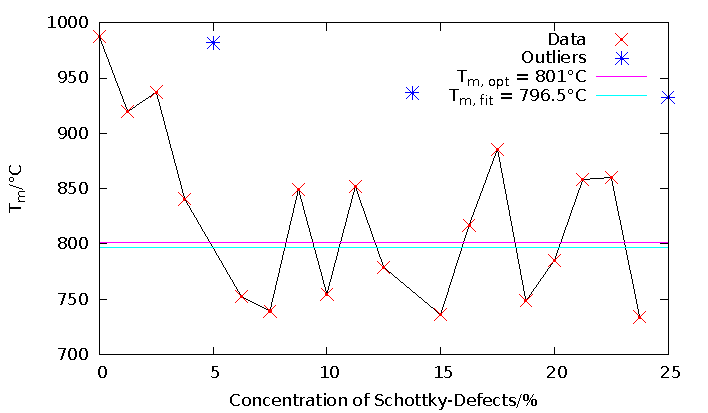
\includegraphics{visuals/nacl_melting.pdf}
    \caption{Melting points at different defect concentrations.
        $T_\textrm{m, opt}$ is the melting point according to literature,
        $T_\textrm{m, fit}$ is the mean value of the oscillating region.
        The black dot-connecting line and outliers are for visualization
    purposes only.}
\end{figure}

The oscillating region starts after \SI{7.5}{\percent}, the resulting
mean value differs by \SI{4.5}{\kelvin} from the exact value of
\SI{801}{\celsius}, which is a relative error as low as
\SI{0.6}{\percent}.

\section{The EAM potential - Observing phase transition in Metall}

The ``embedded atom method'' (EAM) is a standard potential used in the analysis of metalls and alloys.
They are used quite successfully in the investigation of fractures, surface reactions martensite-austenite transitions
and phasechanges in condensed matter, nano particles and thin films.

In this tutorial lesson we will demonstrate the use of the EAM potential and how a phase transition
can be analyzed with Tremolo-X. 
We will heat a Fe-Ni nanoparticle from 100 K to 800 K and observe it changing its lattice structure from
bcc to fcc/hcp.

In order to use EAM potentials, the user must have a file with EAM parameters in the format ``eam/fs'' (a generalized EAM type by Finnis-Sinclaire) or 
in the ``eam/alloy'' format, which is slightly modified from DYNAMO setfl file formats. For a detailled description of the EAM formats supported, please
check the appropriate section \ref{potentials:eam}

The unit system of the eam parameters file determines the units which need to be used throughout the simulation. As a result in this example SI units will be used.
The respective entries for iron and nickel particle values in the potential file are consequently:
\begin{lstlisting}
particles	{
	particle:	particle_type=Fe,	element_name=Fe,	
			sigma=1.0,		epsilon=0.0,	
			sigma14=1.0,		epsilon14=0.0,	
			mass= 9.2732785e-26,	
			free=3,
			charge=0;
	particle:	particle_type=Ni,	element_name=Ni,	
			sigma=1.0,		epsilon=0.0,	
			sigma14=1.0,		epsilon14=0.0,	
			mass=9.7462664e-26,	
			free=3,
			charge=0;
	};	
\end{lstlisting}

and subsequently we specify the format (``alloy'' format) and the filename in the following way:
\begin{lstlisting}
eam    {
         setfl:     file="Fe-Ni-MeyerEntel-1995.eam.alloy";        
       };
\end{lstlisting}


In the parameter file we need to specify the following:

\begin{lstlisting}
integration: type=dynamics;
########## Section Domain:
domain {
      size:    type=cube, size=60.0e-10;
      border:  bt_xlow=periodic,
               bt_xhigh=periodic,
               bt_ylow=periodic,
               bt_yhigh=periodic,
               bt_zlow=periodic,
               bt_zhigh=periodic;
		};
########## Section Ensemble and Propagator:
dynamics {
	ensemble:	ensemble=NVT;
	propagator,	verlet:	delta_T=1.0e-15,	endtime=8.0e-11,	timeinteps=1e-07,	maxiteration=100;
	thermostat	{
		berendsen:  state=on,
                            T_Interval=1.0e-15;
		timeline:   state=on,
                      [time, temperature, interpolation=
		      (0,        1.3806503e-21, linear), # 100K / 7.2429638e+22 K
	              (1e-14,	 1.3806503e-21,	linear),
		      (7.56e-11, 1.1045202e-20,	linear), # 800K
		      (8.0e-11,	 1.1045202e-20,	linear)];
			};
	 };
########## Section Solver and Parallelization:
lcs:	cellrcut=5.6001e-10; 
########## Section Output Measurement:
output	{
	Outvis:	T_Start=0, T_Delta=5.0e-13, Step_Delta=100;
	Outm:	T_Start=0, T_Delta=1.0e-15, Step_Delta=100;
	Outmm:	T_Start=0, T_Delta=5.0e-14, T_Deltam=4.0e-14, Step_Delta=20, Step_Deltam=10;
	Outdata: T_Start=0, T_Delta=10.0e-13, Step_Delta=50;
	energy:	measure=on,	meanmeasure=off;
	analyze	{
	  radial: measure=on, meanmeasure=off, vis=on, r_cut=5.6001e-10, n_bin=56;
		radialdistribution	{
	            radialdist: particle_type1=Ni, particle_type2=Ni;
		    radialdist: particle_type1=Ni, particle_type2=Fe;
        	    radialdist: particle_type1=Fe, particle_type2=Fe;
                     };
                   };
	};
\end{lstlisting}

Note that while we use SI units, the temperature has a scaling prefactor, which needs to be accounted for when setting the thermostat. While we use periodic boundaries, those will not be relevant to our simulation, as we 
set the simulation domain to a cube of 60$\angstrom$, whereas the nanoparticle has a radius of 20 $\angstrom$. Thus no interaction with or across the domain boundaries is present.

We now can run the simulation.After having run the simulation, we can take a look at the potential energy curve and notice that its slope changes around 4.64e-11s into the simulation. It is at this time that
the transformation takes place.

We will now analyze the radial distribution of the sample at the beginning of the simulation, during the melting phase and after the transition phase.
For this we will use the tool ``CalcRadialHist'' delivered with Tremolo-X.

By calling 
\begin{lstlisting}
CalcRadialHisto eam.histogram 5e-15 15.3e-15 0.0 5.6e-10 3.0e-10 1 56 545 2196 216000 3.0e-10 > RadialHist
\end{lstlisting}
we average the radial distribution over the time interval from 5 to 15 fs and write the results to the file {\tt RadialHist}.
The same can be done for the time intervals 4e-11s to 4.3e-11s and  5e-11s to 5.3-11s. When those three distributions are compared,
we observe, that around 4e-11s the original configuration has been severly melted, but that around 5e-11s the atoms have rearanged themselves, 
which can be seen from the clearly shifted peaks in the radial distribution function.



